 % easychair.tex,v 3.2 2012/05/15
%
% Select appropriate paper format in your document class as
% instructed by your conference organizers. Only withtimes
% and notimes can be used in proceedings created by EasyChair
%
% The available formats are 'letterpaper' and 'a4paper' with
% the former being the default if omitted as in the example
% below.
%
\documentclass{easychair}
%\documentclass[debug]{easychair}
%\documentclass[verbose]{easychair}
%\documentclass[notimes]{easychair}
%\documentclass[withtimes]{easychair}
%\documentclass[a4paper]{easychair}
%\documentclass[letterpaper]{easychair}

% This provides the \BibTeX macro
\usepackage{doc}
\usepackage{makeidx}
\usepackage{tikz}
\usetikzlibrary{shapes,arrows}
\usepackage{graphicx}
\usepackage{amstext}    % defines the \text command, needed here
\usepackage{array} 
\usepackage{listings}
\usepackage{latexsym}
\usepackage{subfigure}
\usepackage{amsmath}
\usepackage{url}
\usepackage{enumitem}
\usepackage{xspace}
\setenumerate{listparindent=\parindent}
\newcommand{\eg}{\emph{e.g.}\xspace}
\newcommand{\figref}[1]{Figure~\ref{#1}}
\newcommand{\listref}[1]{Listing~\ref{#1}}

\tikzstyle{decision} = [diamond, draw, fill=red!20, 
    text width=6em, text badly centered, node distance=3cm, inner sep=0pt]
\tikzstyle{block} = [rectangle, draw, fill=blue!20, 
    text width=5em, text centered, rounded corners, minimum height=4em]

\tikzstyle{redblock} = [rectangle, draw, fill=red!20, 
    text width=5em, text centered, rounded corners, minimum height=4em]
\tikzstyle{greenblock} = [rectangle, draw, fill=green!20, 
    text width=5em, text centered, rounded corners, minimum height=4em]
\tikzstyle{line} = [draw, -latex']
\tikzstyle{cloud} = [draw, ellipse,fill=blue!20, node distance=3cm,
    minimum height=2em]
\tikzstyle{circle} = [draw, circle,fill=blue!20, node distance=3cm,
    minimum height=2em]

% In order to save space or manage large tables or figures in a
% landcape-like text, you can use the rotating and pdflscape
% packages. Uncomment the desired from the below.
%
% \usepackage{rotating}
% \usepackage{pdflscape}

% If you plan on including some algorithm specification, we recommend
% the below package. Read more details on the custom options of the
% package documentation.
%
% \usepackage{algorithm2e}

% Some of our commands for this guide.
%
\newcommand{\easychair}{\textsf{easychair}}
\newcommand{\miktex}{MiK{\TeX}}
\newcommand{\texniccenter}{{\TeX}nicCenter}
\newcommand{\makefile}{\texttt{Makefile}}
\newcommand{\latexeditor}{LEd}

%\makeindex

%% Document
%%
\begin{document}

%% Front Matter
%%
% Regular title as in the article class.
%
\title{Variability Modeling in Clafer Using SMT}

% \titlerunning{} has to be set to either the main title or its shorter
% version for the running heads. When processed by
% EasyChair, this command is mandatory: a document without \titlerunning
% will be rejected by EasyChair

\titlerunning{Variability Modeling in Clafer Using SMT}

% Authors are joined by \and. Their affiliations are given by \inst, which indexes
% into the list defined using \institute
%
\author{
Ed Zulkoski\\
}

% Institutes for affiliations are also joined by \and,
\institute{
  University of Waterloo,
  Waterloo, Ontario, Canada\\
  \email{ezulkosk@gsd.uwaterloo.ca} \\
  (ezulkosk, 20456819) \\
 }
%  \authorrunning{} has to be set for the shorter version of the authors' names;
% otherwise a warning will be rendered in the running heads. When processed by
% EasyChair, this command is mandatory: a document without \authorrunning
% will be rejected by EasyChair

\authorrunning{Zulkoski}


\clearpage

%%%%%%%%%%%%%%%%%%%%%%%%%%%%%%%%%%%%%%%%%%%%%%%%%%%
\maketitle
%%%%%%%%%%%%%%%%%%%%%%%%%%%%%%%%%%%%%%%%%%%%%%%%%%%

\begin{abstract}
We present a new backend for Clafer - a variability modeling language - using the Z3 Satisfiability Modulo Theory (SMT) solver. Z3 is well respected for its speed and has been shown to outperform other solvers in the domain of partial modeling -- one type of modeling within the scope of Clafer. We show that, by retaining the notion of a $scope$, Clafer can generally be expressed within the logic of \texttt{QF\_UFNRA} (quantifier-free non-linear real arithmetic), however all Clafer models encountered so far can be expressed in \texttt{QF\_LIA} (quantifier-free linear integer arithmetic). We are capable of supporting language features not previously available in Clafer, including constraints over real numbers, and string constraints, leveraging Z3-Str: a theory extension to Z3. We conclude with a discussion of other extensions we have made, as well as new directions for future work that would not be possible with other Clafer backends.
\end{abstract}

\setcounter{tocdepth}{2}
{\small
\tableofcontents}

%\section{To mention}
%
%Processing in EasyChair - number of pages.
%
%Examples of how EasyChair processes papers. Caveats (replacement of EC
%class, errors).

\pagestyle{empty}


%------------------------------------------------------------------------------
\section{Introduction}
Clafer is a modeling language with first-class support for feature and meta-modeling \cite{BakClafer}. In earlier work, Clafer has been translated to two backend solvers 1) Alloy -- a bounded relational model checker, and 2) Choco -- a library for constraint satisfaction problems. A Clafer specification can be translated to either of these two backends, which produce models of the specification if it is satisfiable, or produce an unsatisfiable core otherwise. Depending on the type of constraints within the Clafer specification, one backend may be more suitable than the other. For example, Alloy does not perform well on arithmetic constraints over large integers, as it deals with them by flattening bounded integer ranges into boolean formulas, however the Choco solver is much more capable in this regard. Still, Choco requires some bounding on integer ranges to facilitate the search process.\\
\indent Furthermore, some desirable language features, such as constraints over real numbers and strings, are not currently supported by either backend due to restrictions of the solvers. Many domains require real numbers to be modeled naturally. For example, any models involving probabilities or percentages can be modeled using reals. One applicable domain that has previously been modeled in Clafer is that of banking. The work investigated the family of available Scotiabank mortgage options, which include interest rates and monetary amounts, both of which can be naturally modeled with reals\footnote{See \url{http://gsd.uwaterloo.ca/node/356}.}. However, due to restrictions of previous backends, the specification could not be instantiated. Clafer should be capable of analyzing these models. \\
\indent In short, the restrictions of Clafer are intrinsically tied to the limitations of its backend solver. In order to address some of these restrictions, we have developed a new translation from Clafer to Z3 \cite{Moura} -- a state-of-the-art SMT solver. Z3 is well known to be a fast solver, motivating our desire to create a new Clafer backend with it. In an experiment by \cite{Saadatpanah2012}, randomly generated partial models were analyzed by four solvers: Alloy, a relational logic solver; Minizinc, a  \textit{constraint satisfaction problems} (CSP) solver; Clasp with GrinGo, an \textit{answer set programming} (ASP) solver; and Z3. Z3 was shown to be more efficient (based on solving time) in general, and also scaled better to harder problems. Z3 has also been shown to perform well relative to other SMT solvers, winning the SMTCOMP 2012 competition in the theory categories of \texttt{QF\_UFLIA}, \texttt{QF\_UFLRA}, and \texttt{QF\_BV}, among others\footnote{Results can be found at \url{http://www.smtexec.org/exec/?jobs=1004} .}. Further, a recent extension to Z3: Z3-Str \cite{Zheng2013}, allows support for some string constraints (\eg length, substring).\\
\indent This paper makes the following contributions:
\begin{enumerate}
\item We describe how Clafer models can be reduced to constraints in logics supported by Z3. 
\item We have developed a tool called \textit{ClaferZ3} that reflects the translation described in this work, and can be found at \url{https://github.com/gsdlab/ClaferZ3}.
\item Our tool supports constraints over real numbers and strings, which are not supported by previous Clafer backends, and thus expands the scope of models that Clafer can analyze. Furthermore, integer instances are unbounded.
\item We discuss further extensions to Clafer that are possible with an SMT backend. For example, we have prototyped a new approach for eliminating isomorphic models (Section \ref{isomorphism}).
%\item We demonstrate that our tool is sufficient to handle string constraints found in eCos models.  
\end{enumerate}

\section{Clafer Overview}
\label{claferoverview}

\emph{Clafer} is a structural modeling language which is designed for variability modeling. It unifies both feature models  and meta-models \cite{BakClafer}. Clafer specifications are built of components called clafers. \\
%
\indent In Listing \ref{listing:ClaferPhone}  we show a specification of two mobile phones in Clafer. 
%
 \texttt{Phone} is an example of a top-level (non-nested) abstract clafer. \textbf{Abstract clafers} do not get directly instantiated in the resulting model, however concrete clafers, such as BudgetPhone and SmartPhone, can extend abstract clafers to inherit their sub-clafers. \textbf{Sub-clafers} are indicated by indentation, and cannot exist without their parent. Although our example only has two levels of indentation, other specifications may have more. The * after \texttt{Phone} indicates that zero or more \texttt{Phone}s may be included in the resulting model. \texttt{Phone} has an optional feature \texttt{Wifi}, denoted by the question mark after it. \texttt{instApps} is a \textbf{reference clafer} (denoted by the  -$>$ symbol) that refers  to a set of installed \texttt{App}s. We emphasize that this is a set: an implicit constraint is that the same phone cannot have two of the same \texttt{App}. However, \textit{different} phones may install the same \texttt{App}. A \texttt{Phone}, has a final attribute of \texttt{cost}, which we indicate is of type real number. Note that clafers that are declared primitive (int/string/real) get \textit{desugared} into reference clafers that point to instances of their respective type. On line 6,  \texttt{App}  is an example of a \textbf{concrete clafer}.\\
%
\indent On line 9, we introduce the concrete clafer \texttt{BudgetPhone}, which inherits all subclafers from \texttt{Phone}. The number 2 after it indicates that their must be exactly two \texttt{BudgetPhone}s in the resulting model. \texttt{BudgetPhone} has two constraints associated with it on lines 10-11 (indicated by square brackets). Line 10 consists of a quantified formula (with quantifier \textit{no}), indicating that a \texttt{BudgetPhone} cannot have \texttt{App}s. Note that this constraint must be true of \textit{all} \texttt{BudgetPhone} instances, due to its level of indentation. Line 11 indicates the price of \texttt{BudgetPhone}s, constraining the inherited clafer \texttt{cost}. Line 14 restricts the cost of \texttt{SmartPhone}s to be its original cost, plus the sum of all installed \texttt{App}s. The dot character in ``instApps.appCost''  in essence serves as a navigation operator, by performing a join between the set of \texttt{App}s associated with this individual \texttt{SmartPhone} and the \texttt{appCost}s associated with them. A model of the specification is given in Listing \ref{listing:ClaferPhoneInstance}.\\ %As a final note, each instance of an abstract clafer can only be instantiated by one instance concrete clafer (\eg \textit{BudgetPhone0} and \textit{BudgetPhone1} cannot both instantiate \textit{Phone0}).
\indent This example only illustrates a fragment of the expressions supported by Clafer. Most notably, set operations such as intersection and union allow richer expressions over instances of clafers. We describe the other components of the language in Section \ref{detailedsolution}

\lstdefinelanguage{clafer}
{morekeywords={abstract, xor, or, integer, min, max, sum},
sensitive=true,
basicstyle={\sffamily\small},
tabsize=2,
columns=fullflexible
}


\begin{figure}[!t]
\par\noindent
\begin{minipage}[t]{.33\textwidth}
\begin{lstlisting}[language=clafer, numbers=left, caption=Clafer specification of two types of phones and apps., label={listing:ClaferPhone}]
abstract Phone *
	Wifi  ?
	instApps ->  App *
	cost : real

App *
	appCost : real

BudgetPhone: Phone 2
	[ no instApps && no Wifi ]
	[ cost = 49.99 ]	

SmartPhone: Phone 1
	[ cost = 99.99 + sum(instApps.appCost)]	
 
\end{lstlisting}%
\end{minipage}%
\hfill
\begin{minipage}[t]{.32\textwidth}
\begin{lstlisting}[language=clafer, caption=A generated model of a mobile phone and its apps in Clafer., label={listing:ClaferPhoneInstance}]
  App0
	  appCost = 0.99
  App1
	  appCost = 2.99
  BudgetPhone0 : Phone0
	  Wifi0
	  cost = 49.99
  BudgetPhone1 : Phone1
  	  cost = 49.99
  SmartPhone0 : Phone2
	  Wifi1
	  instApps0 -> App0
	  instApps1 -> App1
	  cost = 103.97
\end{lstlisting}%
\end{minipage}%
\hfill
\begin{minipage}[t]{.32\textwidth}
\begin{lstlisting}[language=clafer, caption=The variables associated with each clafer in Z3\, corresponding to Listing 2., label={listing:ClaferPhoneZ3}]


Phone: [0, 0, 0]
Wifi: [0, 2, 3]
instApps: [2, 2, 3]
instApps_ref: [0, 1, 3]
cost: [0, 1, 2]
cost_ref: [49.99, 49.99, 103.97]
App: [0, 0, 1]
appCost_ref: [0.99, 2.99, 0]
BudgetPhone: [0, 0]
SmartPhone: [0]
\end{lstlisting}%
\end{minipage}%
\end{figure}

%\begin{figure}[!t]
%\centering
%	\subfigure{
% \begin{lstlisting}[language=clafer]
%Phone0
%	Wifi0
%	Apps0 ->  SwApps0
%	Apps1 ->  SwApps1
%	
%SwApps0 
%	UID0=5
%	memory1=15
%
%SwApps1 
%	UID1=6
%	memory1=26
%  \end{lstlisting}
%	}
%	\subfigure{
% \begin{lstlisting}[language=clafer]
%Phone0
%	Wifi0
%	Apps0 ->  SwApps0
%	Apps1 ->  SwApps1
%	
%SwApps0 
%	UID0=5
%	memory1=15
%
%SwApps1 
%	UID1=6
%	memory1=26
%  \end{lstlisting}	
%}
%\caption{A specification for a mobile phone and its apps  in Clafer (left), a  generated model that satisfies such specification (center) and  the computed scopes  of each entity in the specification (right).}
%\label{fig:AllFiguresClafer}
%\end{figure}

%
%\begin{figure}[]
% \begin{lstlisting}[language=clafer]
%
%
%Phone0
%	Wifi0
%	Apps0 ->  SwApps0
%	Apps1 ->  SwApps1
%	
%SwApps0 
%	UID0=5
%	memory1=15
%
%SwApps1 
%	UID1=6
%	memory1=26
%  \end{lstlisting}
% \caption{ \figref{fig:ClaferPhone} }
% \label{fig:ClaferPhoneInstance}
%\end{figure}


\section{Solution Overview}

\begin{figure}
\centering
\label{claferZ3toolchain}
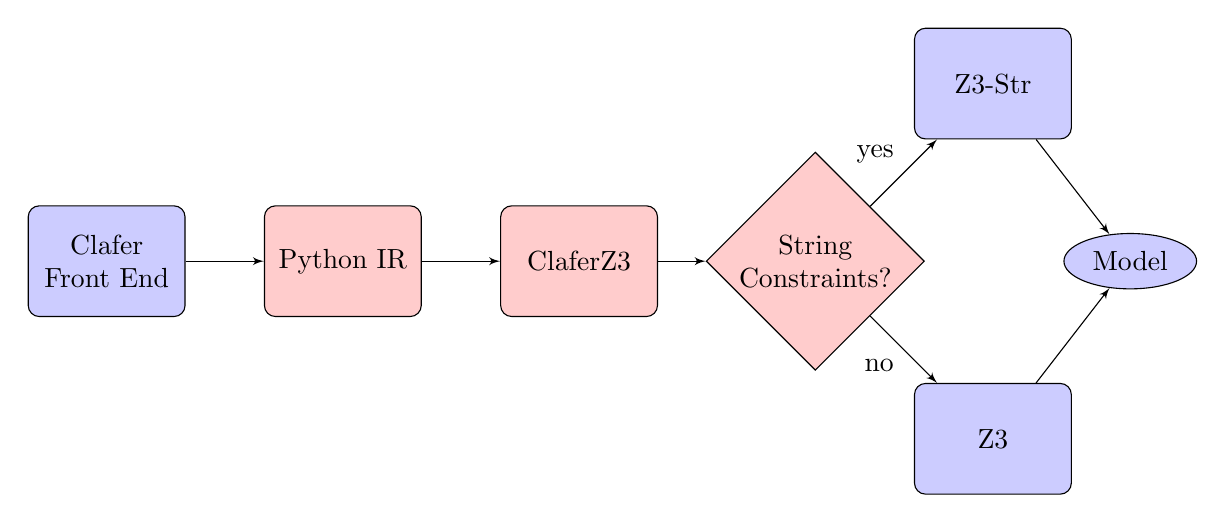
\begin{tikzpicture}[node distance = 3cm, auto]
    % Place nodes
    \node [block] (FrontEnd) {Clafer Front End};
    \node [redblock, right of=FrontEnd] (PythonIR) {Python IR};
    \node [redblock, right of=PythonIR] (ClaferZ3) {ClaferZ3};
    %\node [block, below of=init] (identify) {identify candidate models};
    %\node [block, below of=identify] (evaluate) {evaluate candidate models};
    %\node [block, left of=evaluate, node distance=3cm] (update) {update model};
    \node [decision, right of=ClaferZ3] (Decision) {String Constraints?};
    \node [block, above right of=Decision, node distance = 3.19cm] (Z3Str) {Z3-Str};
    \node [block, below right of=Decision, node distance = 3.19cm] (Z3) {Z3};
    \node [cloud, right of=Decision, node distance = 4cm] (Model) {Model};
    %\node [block, below of=decide, node distance=3cm] (stop) {stop};
    % Draw edges
    \path [line] (FrontEnd) -- (PythonIR);
    \path [line] (PythonIR) -- (ClaferZ3);
    \path [line] (ClaferZ3) -- (Decision);
    %\path [line] (evaluate) -- (decide);
    \path [line] (Decision) -- node[below left] {no} (Z3);
\path [line] (Decision) -- node {yes} (Z3Str);
\path [line] (Z3) --  (Model);
\path [line] (Z3Str) --  (Model);
    %\path [line] (update) |- (identify);
    %\path [line] (decide) -- node(stop);
   
  %  \path [line,dashed] (system) |- (evaluate);
\end{tikzpicture}
\caption{Depicts ClaferZ3 within the Clafer toolchain. Nodes marked red indicate contributions of this work.}
\end{figure}
We describe the approach of our translation through our example in Section \ref{claferoverview}. For consistency (and due to large amounts of overlapping terminology), we define the following terms and notations: 1) we use capitalized \textit{Clafer} to denote the language Clafer itself, and lowercase \textit{clafer} to denote individual components of the input (\eg \texttt{Phone} in Listing \ref{listing:ClaferPhone}); 2) we call the Clafer input the \textit{specification} (\eg Listing \ref{listing:ClaferPhone}); 3) an output that conforms to the specification is a \textit{model} (e.g. Listing \ref{listing:ClaferPhoneInstance}); and 4) individual occurrences of a clafer in the model are \textit{instances} (\eg \textit{Phone0} in Listing \ref{listing:ClaferPhoneInstance}). \\
\indent Figure \ref{claferZ3toolchain} depicts how our translation of Clafer to Z3 fits into the Clafer toolchain. Clafer specifications are first run through the front-end (scanner, parser, type-checker, etc.), and a representation of the input is generated in Python. Using the Z3Py API, ClaferZ3 generates a set of variables and asserts constraints over them. If string constraints are not present, then we can use the standard Z3 implementation to check for satisfiability, else we use Z3-Str.  If the solver finds a satisfying assignment over the generated variables and constraints, then the values of these variables can be interpreted as a Clafer model. \\
\indent We devote the remainder of this section to describing the variables generated to express our Clafer specification in Z3, and how their valuations are interpreted back into a Z3 model. The actual constraints over the variables are discussed in Section \ref{detailedsolution}. We hope that by discussing the end result first, the constraint that need to be generated are more intuitive.
\subsection{Interpreting Z3 output as a Clafer Model}

%\indent The logic of Clafer can essentially be reduced to the following main components:
%\begin{itemize}
%\item Finite sets, and operations over them (e.g. set union). For the translation to Z3, we use a finite list of bounded integer variables to represent a given clafer\footnote{Since our integers have bounded ranges,  bitvectors should be sufficient as well, and may increase performance. We discuss this in Section \ref{FutureWork}.}. Abstractly, each integer in the list corresponds to a \textit{potential} instance of that clafer in the outputted model. An instance is part of the model if Z3 returns a value for it not equal to a predefined \textit{sentinel} number for that clafer (more details are further described in the following section). We then need to add constraints over these sets, such that if a satisfying assignment is returned from Z3 for these variables, then it can be mapped back to a Clafer model conforming to the specification. For example, these constraints must ensure that the number of instances of a clafer are within the specified cardinality, and that all bracketed constraints are satisfied.
%\item Basic arithmetic constraints (e.g. addition, multiplication) and boolean constraints (e.g. \textit{and}, \textit{or}, \textit{not}), which have direct translations to Z3.
%\end{itemize} 

%Most of the difficulty lies in creating constraints over the finite sets in such a way that the integer variables can be mapped to a model conformant to the specification. We discuss some details of this next.


%\begin{figure}[!t]
%\centering
%\begin{lstlisting}[language=clafer, caption=A more complex mobile phone specification in clafer., label={listing:ClaferMoreComplexSpec}, xleftmargin=.2\textwidth, xrightmargin=.2\textwidth]
%SwApps *
%	memory : int

%IPhoneApps -> SwApps *	
%	[ this.ref.memory < 15 ]
%AndroidApps -> SwApps *

%[ sum AndroidApps.ref.memory <= 100 ]	
%\end{lstlisting}%
%\end{figure}


\section{Detailed Solution Overview}
\label{detailedsolution}
%We illustrate some components of our approach through the example Clafer specification and instance in Listings \ref{listing:ClaferPhone} and \ref{listing:ClaferPhoneInstance}, respectively. Note that there are many aspects of Clafer not present in this model, such as abstract clafers and inheritance; we reserve a description of these for the final report.
This section describes the Z3 constraints that are generated to represent a Clafer specification in Z3. We begin with our representation of a clafer in Section \ref{representation}. The remaining sections constrain this representation to conform to all restrictions of the specification (\eg cardinality constraints, bracketed constraints, etc.).

\subsection{Representation of a clafer}
\label{representation}
We borrow two key ideas from a previous translation of Clafer to Choco \cite{jimmy}: 1) clafers are represented as a finite number of integers; and 2) clafers that extend abstract clafers have a direct mapping to their supers (we discuss this point later).\\
\indent We reprensent a clafer as a finite list of integers. Consider the \texttt{Phone} clafer in Listing \ref{listing:ClaferPhone}. Since our outputted Clafer model will have at most two \texttt{Phone} clafers, we can represent it with a list of two integer variables, say $[phone0, phone1]$.  \\
\indent For star-cardinalities (as in the reference clafer \texttt{Apps}), we place a finite \textit{scope} $s$ on the clafer, indicating that only $s$ instances can occur in the model. For the sake of example, let us assume that the scope of all unbounded clafers is $4$. Then we can represent the clafer \texttt{Apps} with the list $[Apps0, Apps1, Apps2, Apps3]$.\\
\indent Semantically, the values of these integer variables represent \textit{parent pointers}, indicating where the clafer should be placed in the outputted model. For example, if the variable $Apps0$ is set to $0$ by the solver, then it should fall directly beneath $Phone0$ in the hierarchy of the outputted model. Likewise, if $Apps0 = 1$, then $Apps0$ would be placed under $Phone1$.\\
\indent A clafer instance is \textit{excluded} from the model if its integer variable is set to a pre-defined \textit{sentinel} value, which equals the total number of instance variables of the clafer's parent. For example, since the \texttt{Apps} clafer is directly underneath \texttt{Phone}, and \texttt{Phone} has two instances variables, any \texttt{Apps} instance set to 2 will not be included in the model. In Fig. 1c, since \textit{Apps2} and \textit{Apps3} both equal 2, they do not appear in the model in Fig. 1b. For \textit{top-level clafers} that do not have a parent, the instance is included if its corresponding variable is set to 0, and not included if set to 1. For simplicity in the remainder of the paper, given a clafer \texttt{x}, an instance \textit{$x_i$} is excluded if  $x_i = x_{sentinel}$ ($Apps2 = Apps_{sentinel}$ in our example). \\
\indent Reference clafers (e.g. \texttt{Apps}) require an additional integer variable associated with each instance, which corresponds to where the reference points. For a reference clafer instance $x_i$, we label its reference $x_i\_ref$. For example, in Listing \ref{listing:ClaferPhoneInstance}, $Apps0$ points to $SwApps0$, indicating that $Apps0\_ref$ in the Z3 output equaled 0. Each reference variable is bounded by the number of instances of the referenced clafer. A reference exists \textit{iff} its corresponding clafer exists (e.g. $Apps0 \ne Apps_{sentinel} \Leftrightarrow Apps0\_ref \ne SwApps_{sentinel}$). \\
\indent Integer clafers (\eg memory) can be treated similarly to reference clafers, however their references are unbounded. Also, if an integer clafer is not present in the model, we set its reference to 0 to facilitate other set operations, such as summation. \\
\indent As a larger example, once again consider Listing \ref{listing:ClaferPhoneInstance}, along with the corresponding output of Z3 in Listing \ref{listing:ClaferPhoneZ3}. For space limitations, each line of Listing \ref{listing:ClaferPhoneZ3} corresponds to all instances of the specified clafer; the line ``Apps: [0,0,2,2]'' is shorthand for $Apps0 = 0, Apps1 = 0, Apps2 = 2, Apps3 = 2$. Since $Apps0 = Apps1 = 0$, they are both beneath $Phone0$, however $Apps2$ and $Apps3$ are not present in the model (since $Apps_{sentinel} = 2$). Since $Apps0\_ref = 0$, $Apps0$ must reference $SwApps0$. Furthermore, since $Apps2$ and $Apps3$ are not present in the model, $Apps2\_ref = Apps3\_ref = SwApps_{sentinel}$.

\subsection{Hierarchical and Cardinality Constraints}
asdf
\subsection{Set Constraints}
asdf
\subsection{Quantifiers}
asdf
\subsection{Other Constraints}
asdf
\subsection{Discussion}
sound, incomplete, qflia (mostly)


\subsection{Bracketed Constraints}

We must also support Clafer's bracketed constraints (as in [$sum\text{ }Apps.ref.memory <= 100$] from Listing \ref{listing:ClaferPhone}), which we only discuss at a very high-level. To generate this constraint, we must first compute each of the joins in $Apps.ref.memory$. which is intuitively the set of \texttt{memory} clafers that are beneath any \texttt{SwApp} referenced by an \texttt{Apps} instance. We must then ensure that the sum of this set of \texttt{memory} instances is less than 100. Note that this is indeed the case in our example, since $memory0 + memory1 =   41 \le 100$.\\
\indent Although this example is not too difficult to convert to Z3 constraints, more complicated expressions and language features make set constraints challenging. Consider the specification in Listing \ref{listing:ClaferMoreComplexSpec}. Both \texttt{IphoneApps} and \texttt{AndroidApps} reference \texttt{SwApps}, however when considering the summation on the last line, we must only consider instances of \texttt{SwApps} referenced by instances of \texttt{AndroidApps}. As another example, two previously unmentioned Clafer keywords are \texttt{this} and \texttt{parent}, which essentially allows one to consider each instance of a clafer individually. For example, the constraint: [$this.ref.memory = 15$] in Listing \ref{listing:ClaferMoreComplexSpec}  essentially states that the \texttt{memory} field of any \texttt{SwApp} referenced by an \texttt{IphoneApp} must be equal to 15. This requires us to generate constraints corresponding to \textit{all} individual instances of \texttt{IphoneApp}.

\section{Extensions to Clafer}
A notable difference of using Z3, as opposed to previous backends of Clafer, is its ability to handle constraints on real numbers\footnote{Due to complications with the Clafer frontend grammar, we have only been able to prototype these constraints with small hand-generated models. This also applies to string constraints. These restrictions will be addressed in the near future.}. Z3 handles real numbers naturally, so incorporating constraints over them into our translation required minimal effort. We therefore do not discuss further details. \\
\indent We next briefly describe our extensions allowing string constraints. We also propose a new algorithm to prevent the generation of models that are isomorphic to previously generated models.

\subsection{String Constraints}
String constraints are supported through Z3-Str \cite{Zheng2013}, an extension to Z3 allowing the string expressions, such as concatenation, substring, and cardinality. If the given specification contains string constraints, we translate to Z3-Str instead of Z3. \\
\indent Since we are using the Z3 Python API (which does not support strings), we need to modify our translation to conform to the Z3-Str input format. Our approach is to first purify any strings and string operations present in the AST of the specification. String variables are temporarily replaced with fresh Int variables, and string expressions are replaced with either fresh Int or fresh Boolean variables, depending on the operation (e.g. cardinality is replaced with an Int, whereas substring is replaced with a Boolean). After all other components of the translation finish, the constraints constructed during translation are converted into Z3-Str format, reintroducing strings and string expressions where necessary.

\begin{figure}[!t]
\centering

\end{figure}

\begin{figure}[!t]
\par\noindent
\begin{minipage}[t]{.49\textwidth}
\begin{lstlisting}[language=clafer, caption=A specification with 6 isomorphic models. Below are two example models., label={listing:isospecification}, xleftmargin=.2\textwidth, xrightmargin=.2\textwidth]

AddsToSix 1
  Digit -> int 3
    [this.ref > 0]
  [sum(Digit.ref) = 6]
  
//example model
AddsToSix0
    Digit0 = 1
    Digit1 = 2
    Digit2 = 3

//isomorphic to first model
AddsToSix0
    Digit0 = 2
    Digit1 = 1
    Digit2 = 3    
  
\end{lstlisting}%
\end{minipage}%
\hfill
\begin{minipage}[t]{.49\textwidth}
\begin{lstlisting}[language=clafer, caption=The Clafer constraint restricting all models isomorphic to Listing \ref{listing:isospecification}., label={listing:isoconstraint}]

    [  //note the negation here
    !( #AddsToSix = 1 &&
      (some Digit0 ; Digit1 ; Digit2 : Digit | 
        (some c0_AddsToSix_sort_0 : AddsToSix | 
          #c0_AddsToSix_sort_0.Digit = 3 &&

          Digit0 in AddsToSix0.Digit &&
          Digit1 in AddsToSix0.Digit &&
          Digit2 in AddsToSix0.Digit &&

          "Digit uniqueness constraints" && 

          Digit0.ref = 1 &&
          Digit1.ref = 2 &&
          Digit2.ref = 3
      ))) ]
\end{lstlisting}%
\end{minipage}%
\end{figure}

\subsection{Isomorphic Model Prevention}
\label{isomorphism}
Clafer can produce many models for a given specification, however many models may have the same structure, that is, they are \textit{isomorphic}. While we do not formally define isomorphism of models, intuitively two models are isomorphic if they have the same number of instances of each clafer, the same tree structure, and the graph formed by reference clafers is isomorphic. From a user's viewpoint,  these \textit{redundant} models are not as useful, and should be excluded if possible. Consider Listing \ref{listing:isospecification}. Essentially, this specification requires three unique positive integers, such that their sum is six. There are six unique models (one for each permutation of the numbers 1, 2, and 3), however they are all isomorphic to each other. \\
\indent Suppose the first example model from Listing \ref{listing:isospecification} has been generated. Listing \ref{listing:isoconstraint} is the constraint (in Clafer syntax) that is added to the specification to prevent future models isomorphic to the first. Essentially, each future model either have a different number of clafers (which is not possible due to cardinality constraints), or must have a digit not equal 1, 2, or 3. Note that by using the \textit{some} quantifier, the order of the \texttt{Digit}s is ignored. \\
\indent Although we have only shown a simple example with integers, the approach extends naturally to larger models and reference clafers. This improves upon previous approaches that only look at the tree structure of the model, and cannot detect isomorphism over reference clafers. We note that this approach is possible as Z3 allows pushing new constraints after a solution has been found. Unfortunately, our approach may add an exponential number of constraints, making it infeasible for many specifications. We are still investigating optimizations for this approach.


\section{Experimental Results}
We provide initial experimental results from four sources: 1) the Audi Car Configurator model from \cite{Michel2012}; 2) a simple Clafer specification of a zoo from \cite{Liang}; 3) a PHP script involving string and integer constraints from \cite{Zheng2013}; and 4) the Clafer test suite. The Clafer test suite contains mostly small specifications, however it was useful for checking the proper functionality of our tool. The test suite contains 43 specifications, and we evaluated all but two. The two excluded specifications did not adhere to small design restrictions of our approach, which are reserved for future work\footnote{Essentially, these specifications require instances of abstract clafers to be part of the concrete model.}. \\
\indent Currently, we do not have any larger models in our evaluation, and we plan to address this limitation of our results in the future. However, our evaluation does demonstrate that our tool can properly analyze specifications from a variety of domains, even outside of what would typically be considered variability models (e.g. the PHP script).\\
\begin{figure}
\begin{center}
  \begin{tabular}{ l || c | r }
    \hline
    Specification & Translation Time(s) & Solving Time(s) \\ \hline \hline
    Clafer Test Suite & 10.55 & 0.88 \\ \hline
    Audi Configurator & 0.13 & 0.01 \\ \hline
    PHP Script & N/A & N/A \\ \hline
    Zoo & 0.84 & 0.15 \\
    \hline
  \end{tabular}
\end{center}
\label{resultstable}
\caption{Translation and solving time for each experiment. Note that the Clafer test suite consists of 41 individual specifications. Times are in seconds.}
\end{figure}
\indent All tests were run on a dual core (2.4GHz) laptop with 8GB of RAM, running 64-bit Linux Mint 14. We used Z3 4.3.2 along with Python 3.2 in our experiments. We specified a global scope of 6 for each test, with the exception of the zoo specification, which requires a scope of 9. \\
\indent Table \ref{resultstable} shows the translation and solving time for our set of specifications. Translation time indicates the time required to convert a Clafer specification to a set of Z3 constraints. Solving time indicates how long Z3 takes to find the first satisfying model for each specification. Although the translation is currently a large bottleneck for our approach, it can certainly be optimized. We find that the low solving times for all specifications indicates that our approach is promising.

\section{Related and Previous Work}
\indent The work of Michel et. al. \cite{Michel2012} discusses how configuration problems can be encoded in SMT using TVL \cite{Classen2011} -- a text based feature modeling language similar to Clafer. TVL supports many of the components of feature modeling, including hierarchy, group cardinality, attributes, enums, and cross-tree constraints. However, several aspects of Clafer require extensions to this work. Most notably, set constraints and quantified expressions. \\
\indent  A previous project \cite{Olaechea2013} within the GSD lab was capable of translating a small subset of Clafer to Z3, in order to support attributed feature models for multi-objective optimization. The primary components of Clafer necessary for this domain include hierarchical constraints, fixed-size cardinalities (e.g. [0..1]), and basic arithmetic constraints. This project subsumes that translation by allowing arbitrary Clafer constraints.\\
\indent This work most closely resembles that of \cite{Liang}. Their work translates Clafer to Choco, a CSP language. We have borrowed components from that work, particularly in our representation of clafers and inherited clafers. We are able to extend Clafer with constraints over strings and real numbers, which neither the Choco nor Alloy backend currently support. Z3 also allows us to handle arbitrarily larger integers, which neither of the other backends support. In addition, in the future we intend to extend this project in order to eliminate the need for scopes on unbounded clafers. We discuss this in Section \ref{future}. \\

\section{Future Work}
\label{future}
This project utilized only a small subset of the available features of Z3. For example, Z3 has support for uninterpreted functions and data types. We would like to modify our translation to take advantage of these features. With this approach, we may be able to eliminate the need for scopes in our implementation. The work in \cite{Achraf}, which translates components of Alloy to SMT, and that of \cite{Moura2009}, which discusses some set theoretic operations using the theory of arrays, may be useful starting points for this extension.\\
\indent One particular reason we did not take this approach yet is due to translation efficiency. As an example, in an early version of this project we used an uninterpreted function to represent cardinality constraints. Given a clafer, the function would restrict its instances to conform to the cardinality constraints. By blasting this function into simple arithmetic constraints (which we can do since we have a bounded number of instances), our translation times were significantly decreased\footnote{Although time differences were not recorded, some relatively small specifications required 2-3 additional seconds.}, even for small models. We emphasize that here we are referring to \textit{translation time}; Z3 took approximately the same time to solve models whether or not functions were used.\\
\indent A proper evaluation is necessary to compare the three Clafer backends that are now available. Since each backend was developed independently and contain unique optimizations, this comparison cannot properly evaluate the effectiveness of Alloy/Choco/Z3 as a backend. However, it would be useful to users of Clafer who wish to choose the ideal backend for their application. 
\indent Finally, we intend to further evaluate our extensions for string and real number constraints. Although we currently have models with these constraints, they cannot be properly compiled by Clafer, due to lack of support in the Clafer frontend (see footnote 3). These issues will be addressed in the near future. 

\section{Conclusions}
We have developed a translation from Clafer to Z3. We extend capabilities of Clafer with string constraints using Z3-Str, as well as constraints over real numbers and unbounded integers. Z3's capability to push new constraints to existing specifications allows a new approach to isomorphism detection of Clafer models. Initial results indicate that our approach seems reasonably fast over a variety of specifications, however larger inputs will be needed to validate our results. With the expressive power of Clafer, coupled with the support for new data types, our approach supports the analysis of new domains of models that previous tools are incapable of handling. 



\bibliographystyle{abbrv}
\bibliography{doc}
\end{document}
